%%
% TUM Corporate Design LaTeX Templates
% Based on the templates from https://www.tum.de/cd
%
% Feel free to join development on
% https://gitlab.lrz.de/tum-templates/templates
% and/or to create an issue in case of trouble.
%
% tum-presentation class for scientific talks, thesis presentations, ...
%
%%

%\documentclass[4to3]{tum-presentation}
%\documentclass[navsym]{tum-presentation}
%\documentclass[nothreeliner]{tum-presentation}
%\documentclass[handout,4on1]{tum-presentation}
%\documentclass[handout,2on1]{tum-presentation}
%\documentclass[handout]{tum-presentation}
\documentclass{tum-presentation}
\usepackage[font=small,labelfont=bf]{caption}
\usepackage{wasysym}
\addbibresource{literature.bib}

\title[Shortened Title]{Clustering-Based Sentiment Analysis for Media Agenda Setting}
\subtitle{Opinion Lab Group 2.3, presentation 6}
\author{Wing Sheung Leung, Qiaoxi Liu}
%\institute[]{\inst{1} Department of Electrical and Computer Engineering,
%  Technical University of Munich (TUM)\\
%  \inst{2} Department of Informatics, Technical University of Munich (TUM)}
%\date{International Conference on Mostly Scientific Topics}

\footline{\insertshortauthor~| \inserttitle}

\begin{document}

\begin{frame}[noframenumbering]
  \titlepage
\end{frame}
\begin{frame}
  \frametitle{Milestones}
  \vspace{2cm}
 \includegraphics[width = \textwidth]{figures/timeline.pdf}
  
\end{frame}
\begin{frame}[t]
  \frametitle{Overview}
  \tableofcontents[hideallsubsections]
  %\tableofcontents[sectionstyle=show,subsectionstyle=show,subsubsectionstyle=shaded]
\end{frame}



\section{Stage 1: Generate sentence embeddings with our corpus}

\subsection{1.1 Embeddings}
\subsubsection{XLING sentence-level embeddings}

\subsubsection{Indexing sentences}
\subsection{1.2 Kmeans and Elbow Method}
\subsubsection{sklearn.cluster.MiniBatchKMeans}
\subsubsection{Elbow Method for determining optimal k}

\subsection{1.3 Identifying topics and setting sentiment}
\subsubsection{Generate topword list}%ClarityscoreGenerator vs. word frequency
\subsubsection{Extracting topics form clustering results}
\subsubsection{Assigning sentiment by pre-trained model}


\begin{frame}
  \frametitle{Output from stage 1}
    
  \begin{figure}[t]
    \includegraphics[width = \textwidth]{figures/journey.pdf}
    \end{figure}

\begin{tabular}{lrlrrlrr}
  {} &  global\_id & corpus\_name &  doc\_id &  com\_id &        date &  cluster &  sentiment \\
  
  0 &          0 &     nytimes &       0 &     NaN &  2005-11-01 &        7 &    0.12500 \\
  1 &          1 &     nytimes &       0 &     NaN &  2005-11-01 &        7 &   -0.12500 \\
  2 &          2 &     nytimes &       0 &     NaN &  2005-11-01 &        9 &    0.07500 \\
  3 &          3 &     nytimes &       0 &     NaN &  2005-11-01 &        7 &    0.50000 \\
  4 &          4 &     nytimes &       0 &     NaN &  2005-11-01 &        7 &   -0.03125 \\
 
  \end{tabular}
\end{frame}

\section{Stage 2: Distribution}
\begin{frame}
  \tableofcontents[currentsection,hideallsubsections]
\end{frame}


\subsection{Representing sentiment distribution for single article}

\begin{frame}
  \frametitle{NYTimes: Labeling GMO}
  \includegraphics[width =0.65 \textwidth]{figures/boxplot_nytimes_175.pdf}
  
\end{frame}

\begin{frame}
  \frametitle{NYTimes: Labeling GMO}
  \begin{description}
    \item \textbf{article}:
    \item Whole Foods Market, the grocery chain, on Friday became the first retailer in the United States to require labeling of all genetically modified foods sold in its stores, a move that some experts said could radically alter the food industry. ... Whole Foods, which specializes in organic products, tends to be favored by those types of consumers, and it enjoys strong sales of its private-label products, whose composition it controls. ... He said Whole Foods looked forward to working with suppliers on the labeling.
    \item \textbf{comments}:
    \item  \begin{itemize}
    \item Sometimes genetically modifying food has unintended consequences like bad tasting tomatoes (or worse)
    \item I have a cousin who works at Whole Foods. He is a \textbf{happy} employee and loves it. Thinks it is a great company.
    \item I am not sure if non-GMO foods are \textbf{healthier} to eat but they are certainly better for the environment.
    \item I \textbf{applaud} Whole Foods for at least taking a stand.
    \item consuming red meat is an emotionally charged issue for many people.
    \item The conclusion: "Red meat consumption is associated with an  \textbf{increased risk} of total, heart, and cancer mortality"
    \item Since apples are apparently the most pesticide-ridden fruit, I have gotten to like the more expensive but sweeter ones.
  \end{itemize}
   \end{description}
\end{frame}

\begin{frame}
  \frametitle{Spiegel: Der Skandal um Dioxin }
  \includegraphics[width =0.65 \textwidth]{figures/boxplot_spiegel_112.pdf}
  
\end{frame}
\begin{frame}
  \frametitle{ Spiegel: Der Skandal um Dioxin }
  \begin{description}
    \item \textbf{article}:
    \item Es ist einer der größten Giftskandale der vergangenen Jahre: Bis zu 3000 Tonnen dioxinverseuchtes Fett wurden laut Bundeslandwirtschaftsministerium an 25 Futtermittelhersteller in mindestens vier Bundesländern geliefert. Wo das Gift von dort aus hingelangte und welche Mengen an Nahrungsmitteln belastet sind, ist weitgehend unklar. Verbraucher reagieren zunehmend verunsichert: Der Verkauf von Hühnereiern ist "spürbar" gesunken, teilte die landwirtschaftliche Marktberichterstattungsstelle MEG mit. Welche Gefahren drohen durch die Einnahme von Dioxin? Welche Vorsichtsmaßnahmen können getroffen werden? SPIEGEL ONLINE gibt Antworten auf sieben Fragen.
    \item \textbf{comments}:
    \item  \begin{itemize}
      \item  Der Dioxin-Skandal war  \textbf{hoffentlich nicht der letzte}. Es sollten so viele wie möglich vorkommen.  \textbf{Am besten aber wäre, wenn ein paar Konsumenten nachweislich an solchen oder anderen Giftstoffen in Lebensmitteln sterben.}
      \item 3000 Tonnen verseuchtes Tierfutter - das ist ein Terroranschlag.
      \item Ich kann und will niemandem verbieten Fleisch von deutschen Rindern zu essen.
      \item den gesetzlichen Vorgaben ist so eine Sache.  \textbf{Fahren Sie mal mit einem Fiat 500 mit 80 km/h frontal gegen eine S-Klasse!}. Ihr Vergleich hinkt doch wohl. \textbf{ Wer sich mit Bio-Artikeln überfrisst, stirbt auch. Also sind Bio-Lebensmittel auch lebensgefährlich, wenn man falsch damit umgeht. Guten Appetit.}
      
    \end{itemize}
   \end{description}
\end{frame}

\begin{frame}
  \frametitle{Observed Features}
 
  \begin{itemize}
    \item Spiegel
    \begin{itemize}
      \item news: Kritical (suspection) 
      \item comments:  \textbf{Sarkasmus, irony}, indirect, spreading among more topics 
    \end{itemize}
    \item NYtimes
    \begin{itemize}
      \item news: Tend to be neutral or positive (like an advertisment for stakeholder)
    \item comments: \textbf{straightforward}, clear statement (against or for), benefit or not
      \end{itemize}
  \end{itemize}

\end{frame}
\section{Stage 3 Correlation Analysis}
%\begin{frame}
%  \tableofcontents[currentsection,hideallsubsections]
%\end{frame}
\subsection{3.1 Global Sentiment distribution on NYTimes and Spiegel }
\begin{frame}[shrink]
  \tableofcontents[currentsection,hideallsubsections,sectionstyle=show/shaded,subsectionstyle=show/shaded/hide]
\end{frame}
\subsubsection{Global Sentiment distribution on NYTimes and Spiegel }%ClarityscoreGenerator vs. word frequency
\begin{frame}
  \frametitle{Stage 3: Distribution of articles and comments Overview }
  \framesubtitle{Comments from NYtimes and Spiegel }
  \begin{description}
 \large
 \item NYtimes
    \item 99 out of 327 has comments.
    \item Sentences of comments from each news:
    \item \begin{itemize}
      \item minmax = (3, 2535)
      \item mean = 481.7
      \item median= 216.0
    \end{itemize}
  \end{description}
  \vspace{0.7cm}
  \begin{description}
    \large
    \item Spiegel
       \item 61 out of 152 has comments.
       \item Sentences of comments from each news:
       \item \begin{itemize}
         \item minmax=(8, 23255)
         \item mean = 2309.0
         \item median= 697.0
       \end{itemize}
     \end{description}
\end{frame}

\begin{frame}
  \frametitle{Our distribution is based on...}
  \begin{description}
 \large
    \item To analyse the correlations between news and its comments (sentences-wise), we select the news which has comments.
    \item We filter out the sentences belonging to garbage-aspects.
    \item \begin{itemize}
    \item NYtimes: We pick up all 99 news  (14660 sentences ) with its comments (47691 sentences)
    \item Spiegel: We pick up all 61 news (5689 sentences) with its comments (140855 sentences)
  \end{itemize}
  \end{description}
\end{frame}

\begin{frame}
  \frametitle{3.1.1 Global Sentiment Score Distribution on NYTimes}
  \begin{itemize}
    \item mean(news) = 0.06 > mean(comments) = 0.033
 \end{itemize}
  \begin{columns}
    \column{0.5\textwidth}
    \begin{minipage}[c]{\linewidth}
        \centering
        \includegraphics[width=0.8\linewidth]{figures/overview_all_sentiments_nytimes_news.pdf}
    \end{minipage}
    \column{0.5\textwidth}
    \begin{minipage}[c]{\linewidth}
        \centering
        \includegraphics[width=0.8\linewidth]{figures/overview_all_sentiments_nytimes_comments.pdf}
    \end{minipage}
    
\end{columns}
\end{frame}

\begin{frame}
  \frametitle{3.1.1 Global Sentiment Score Distribution on Spiegel}
  \begin{itemize}
    \item mean(news) = -0.046 > mean(comments) = -0.062
 \end{itemize}
  \begin{columns}
    \column{0.5\textwidth}
    \begin{minipage}[c]{\linewidth}
        \centering
        \includegraphics[width=0.8\linewidth]{figures/overview_all_sentiments_spiegel_news.pdf}
    \end{minipage}
    \column{0.5\textwidth}
    \begin{minipage}[c]{\linewidth}
        \centering
        \includegraphics[width=0.8\linewidth]{figures/overview_all_sentiments_spiegel_comments.pdf}
    \end{minipage}
    
\end{columns}
\end{frame}




\subsubsection{3.1.2 Global Sentiment distribution per topic on Spiegel}
\begin{frame}
  
 
  \frametitle{3.1.2 Global Sentiment distribution per topic on NYTimes}
  \begin{columns}
  \column{0.8\textwidth}
    \begin{minipage}[c]{\linewidth}
      \begin{itemize}
        \item mean:  polarity of one aspect ( red (>0) is postive)
        \item weight: how frequent/how much this aspect are mentioned (all weights sum up to 1 in one article)
        \item quantile: how wide are variety of opinions (diverse range)
     \end{itemize}
  \end{minipage}
  \column{0.2\textwidth}
  \begin{minipage}[c]{\linewidth}
  \includegraphics[width=0.6\linewidth]{figures/legend.pdf}
\end{minipage}
  \end{columns}
  \begin{columns}
    \column{0.5\textwidth}
    \begin{minipage}[c]{\linewidth}
        \centering
        \includegraphics[width=\linewidth]{figures/all_boxplot_all_sentiments_nytimes_news.pdf}
    \end{minipage}
    \column{0.5\textwidth}
    \begin{minipage}[c]{\linewidth}
     
        \centering
        \includegraphics[width=\linewidth]{figures/all_boxplot_all_sentiments_nytimes_comments.pdf}
    
      \end{minipage}
\end{columns}
\end{frame}

\begin{frame}
  \frametitle{3.1.2 Global Sentiment distribution per topic on Spiegel}
  \begin{itemize}
    \item news: left, comments: right
 \end{itemize}
  \begin{columns}
    \column{0.5\textwidth}
    \begin{minipage}[c]{\linewidth}
        \centering
        \includegraphics[width=0.95\linewidth]{figures/all_boxplot_all_sentiments_spiegel_news.pdf}
    \end{minipage}
    \column{0.5\textwidth}
    \begin{minipage}[c]{\linewidth}
        \centering
        \includegraphics[width=0.95\linewidth]{figures/all_boxplot_all_sentiments_spiegel_comments.pdf}
    \end{minipage}
\end{columns}
\end{frame}

\subsubsection{3.1.3 Relation between articles and comments sentiment }
\begin{frame}
  \frametitle{3.1.3 Relation between articles and comments sentiment}
  \begin{itemize}
    \item nytimes: left, spiegel: right
 
 \end{itemize}
  \begin{columns}
    \column{0.5\textwidth}
    \begin{minipage}[c]{\linewidth}
        \centering
        \includegraphics[width=0.95\linewidth]{figures/all_boxplot_combinedall_sentiments_nytimes_news.pdf}
    \end{minipage}
    \column{0.5\textwidth}
    \begin{minipage}[c]{\linewidth}
        \centering
        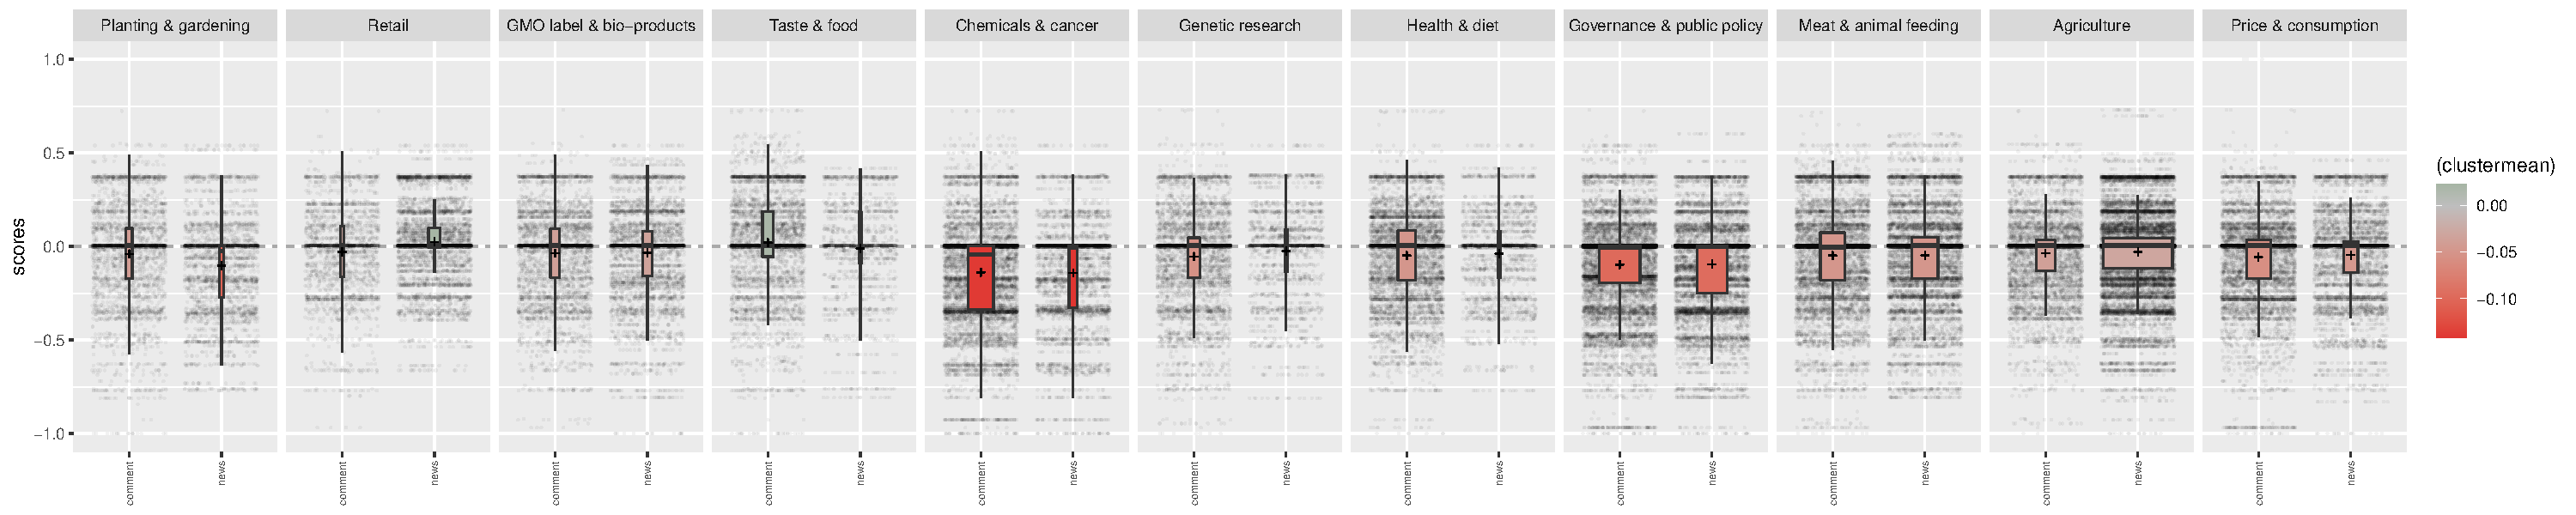
\includegraphics[width=0.95\linewidth]{figures/all_boxplot_combinedall_sentiments_spiegel_news.pdf}
    \end{minipage}
\end{columns}
\end{frame}

\subsection{3.2 Visualization of Correlation of sentiment on NYTimes and Spiegel }
\begin{frame}[shrink]
  \tableofcontents[currentsection,hideallsubsections,sectionstyle=show/shaded,subsectionstyle=show/shaded/hide]
\end{frame}

\subsubsection{3.2.1 Global Relation between number of sentences with sentiment quantile/variance }
\begin{frame}
  \frametitle{3.2.1 Global Relation between number of sentences with sentiment (15\%-85\%)quantile/variance }
  \begin{itemize}
    \item obersavation: quantile/var varies for fewer comments, as the num of sentences of comments increase, it converges.
    \item nytimes (left) : there is no significant relation between the num of sentences and its quantile/var
    \item spiegel (right) : slightly getting larger when num of sentences grows
 \end{itemize}
  \begin{columns}
    \column{0.5\textwidth}
    \begin{minipage}[c]{\linewidth}
        \centering
        \includegraphics[width=0.95\linewidth]{figures/num_commentsentences_var_quantileny_1585_cluster_weight.pdf}
    \end{minipage}
    \column{0.5\textwidth}
    \begin{minipage}[c]{\linewidth}
        \centering
        \includegraphics[width=0.95\linewidth]{figures/num_commentsentences_var_quantilesp_1585_cluster_weight.pdf}
    \end{minipage}
\end{columns}
\end{frame}


\begin{frame}
  \frametitle{3.2.1 Relation between number of sentences with sentiment quantile per topic}
  \begin{itemize}
    \item obersavation: some topics appear only in shorter comments
    \item nytimes (left) per topic: very weak pos-correlation between the num of sentences and its quantile
    \item spiegel (right) per topic: slightly getting larger when num of sentences grows
 \end{itemize}
  \begin{columns}
    \column{0.5\textwidth}
    \begin{minipage}[c]{\linewidth}
        \centering
        \includegraphics[width=0.95\linewidth]{figures/num_commentsentences_quantile_perclusterny_cluster_weight.pdf}
    \end{minipage}
    \column{0.5\textwidth}
    \begin{minipage}[c]{\linewidth}
        \centering
        \includegraphics[width=0.95\linewidth]{figures/num_commentsentences_quantile_perclustersp_cluster_weight.pdf}
    \end{minipage}
\end{columns}
\end{frame}




\subsubsection{3.2.2 Correlation between news and its comments }
\begin{frame}

  \frametitle{3.2.2 Correlation between NYtimes news and its comments}
Variables are means(normally distributed)/weights/quantile . 
\\Apply cor.test(var\_new,var\_comments). Value is its correlation coefficient(pearson,spearman)

  \begin{columns}[t]
    \column{0.7\textwidth}
    \begin{minipage}[c]{\linewidth}
        \centering
        \includegraphics[width=0.85\linewidth]{figures/cor_bar_NYTimes.pdf}
    \end{minipage}
    \column{0.3\textwidth}
    \begin{minipage}[c]{\linewidth}
      \begin{itemize}
        \item \textbf{means} pos correlated: \smiley{} $\rightarrow$ \smiley{} otherwise  \smiley{} $\rightarrow$  \frownie{} 
        \item \textbf{weights} also (highly) pos correlated: the topics in news remain discussed mainly
        \item \textbf{quantile} pos correlated : greater/smaller in news $\rightarrow$ greater/smaller in comments
      \end{itemize}
  \end{minipage}
  \end{columns}
\end{frame}
\begin{frame}
  \frametitle{3.2.2 Correlation between Spiegel news and comments}

  \begin{columns}
    \column{0.7\textwidth}
    \begin{minipage}[c]{\linewidth}
        \centering
        \includegraphics[width=0.95\linewidth]{figures/cor_bar_Spiegel.pdf}
    \end{minipage}
    \column{0.3\textwidth}
    \begin{minipage}[c]{\linewidth}
    \begin{itemize}
      \item \textbf{means} more topics neg correlated  \smiley{} $\rightarrow$  \frownie{} than NYtimes
      \item \textbf{weights} (highly) pos correlated: the topics in news remain discussed mainly. Same as NYtimes
      \item \textbf{quantile} more topics neg correlated : small range variety in news $\rightarrow$ greater (fierce discussion) in comments
    \end{itemize}
  \end{minipage}
\end{columns}
\end{frame}

\section{Top words}
\begin{frame}[fragile]
  \frametitle{Tackled issue on top words selection}
  \begin{itemize}
  \item Problems related to clarity score:
    \begin{enumerate}
        \item Imbalanced existence of English and German words from original top words list 
        \item Incoherent top words among English and German corpus
    \end{enumerate}
  \item Solutions:
    \begin{enumerate}
      \item Pre-processed tokenized sentences
        \begin{itemize}
            \item Replaced URLs with string 'url'
            \item Ignored sentences with length smaller than 15
        \end{itemize}
      \item Re-generated sentence embeddings for pre-processed sentences with XLING
      \item Re-run kmean clustering with the new sentences embeddings
      \item Revised clarity score calculation
        \begin{itemize}
          \begin{lstlisting}
          vectorizer = TfidfVectorizer(stop_words = stopwords, norm = 'l1')
          corpus_bag_of_word = vectorizer.vocabulary_
          corpus_idf = vectorizer.fit(corpus_sentences)
          corpus_tfidf = vectorizer.transform([' '.join(corpus_sentences)]) # i.e. t(w)
    
          # for each cluster
          cluster_vectorizer = TfidfVectorizer(stop_words = stopwords, norm = 'l1', 
                                               vocabulary = corpus_bag_of_word)
          cluster_idf = cluster_vectorizer.fit(cluster_sentences)
          cluster_tfidf = cluster_vectorizer.transform([' '.join(cluster_sentences)]) # i.e. t_a(w)
          \end{lstlisting}
        \end{itemize}
    \end{enumerate}
  \end{itemize}
\end{frame}

\begin{frame}
  \frametitle{k = 15 is optimal from AIC plot}
  \begin{figure}[t]
      \includegraphics[width=0.8\textwidth]{images/AICs_combined.png}
  \end{figure}
\end{frame}

\begin{frame}
  \frametitle{English and German top words are coherent when k =15}
  \begin{figure}[t]
      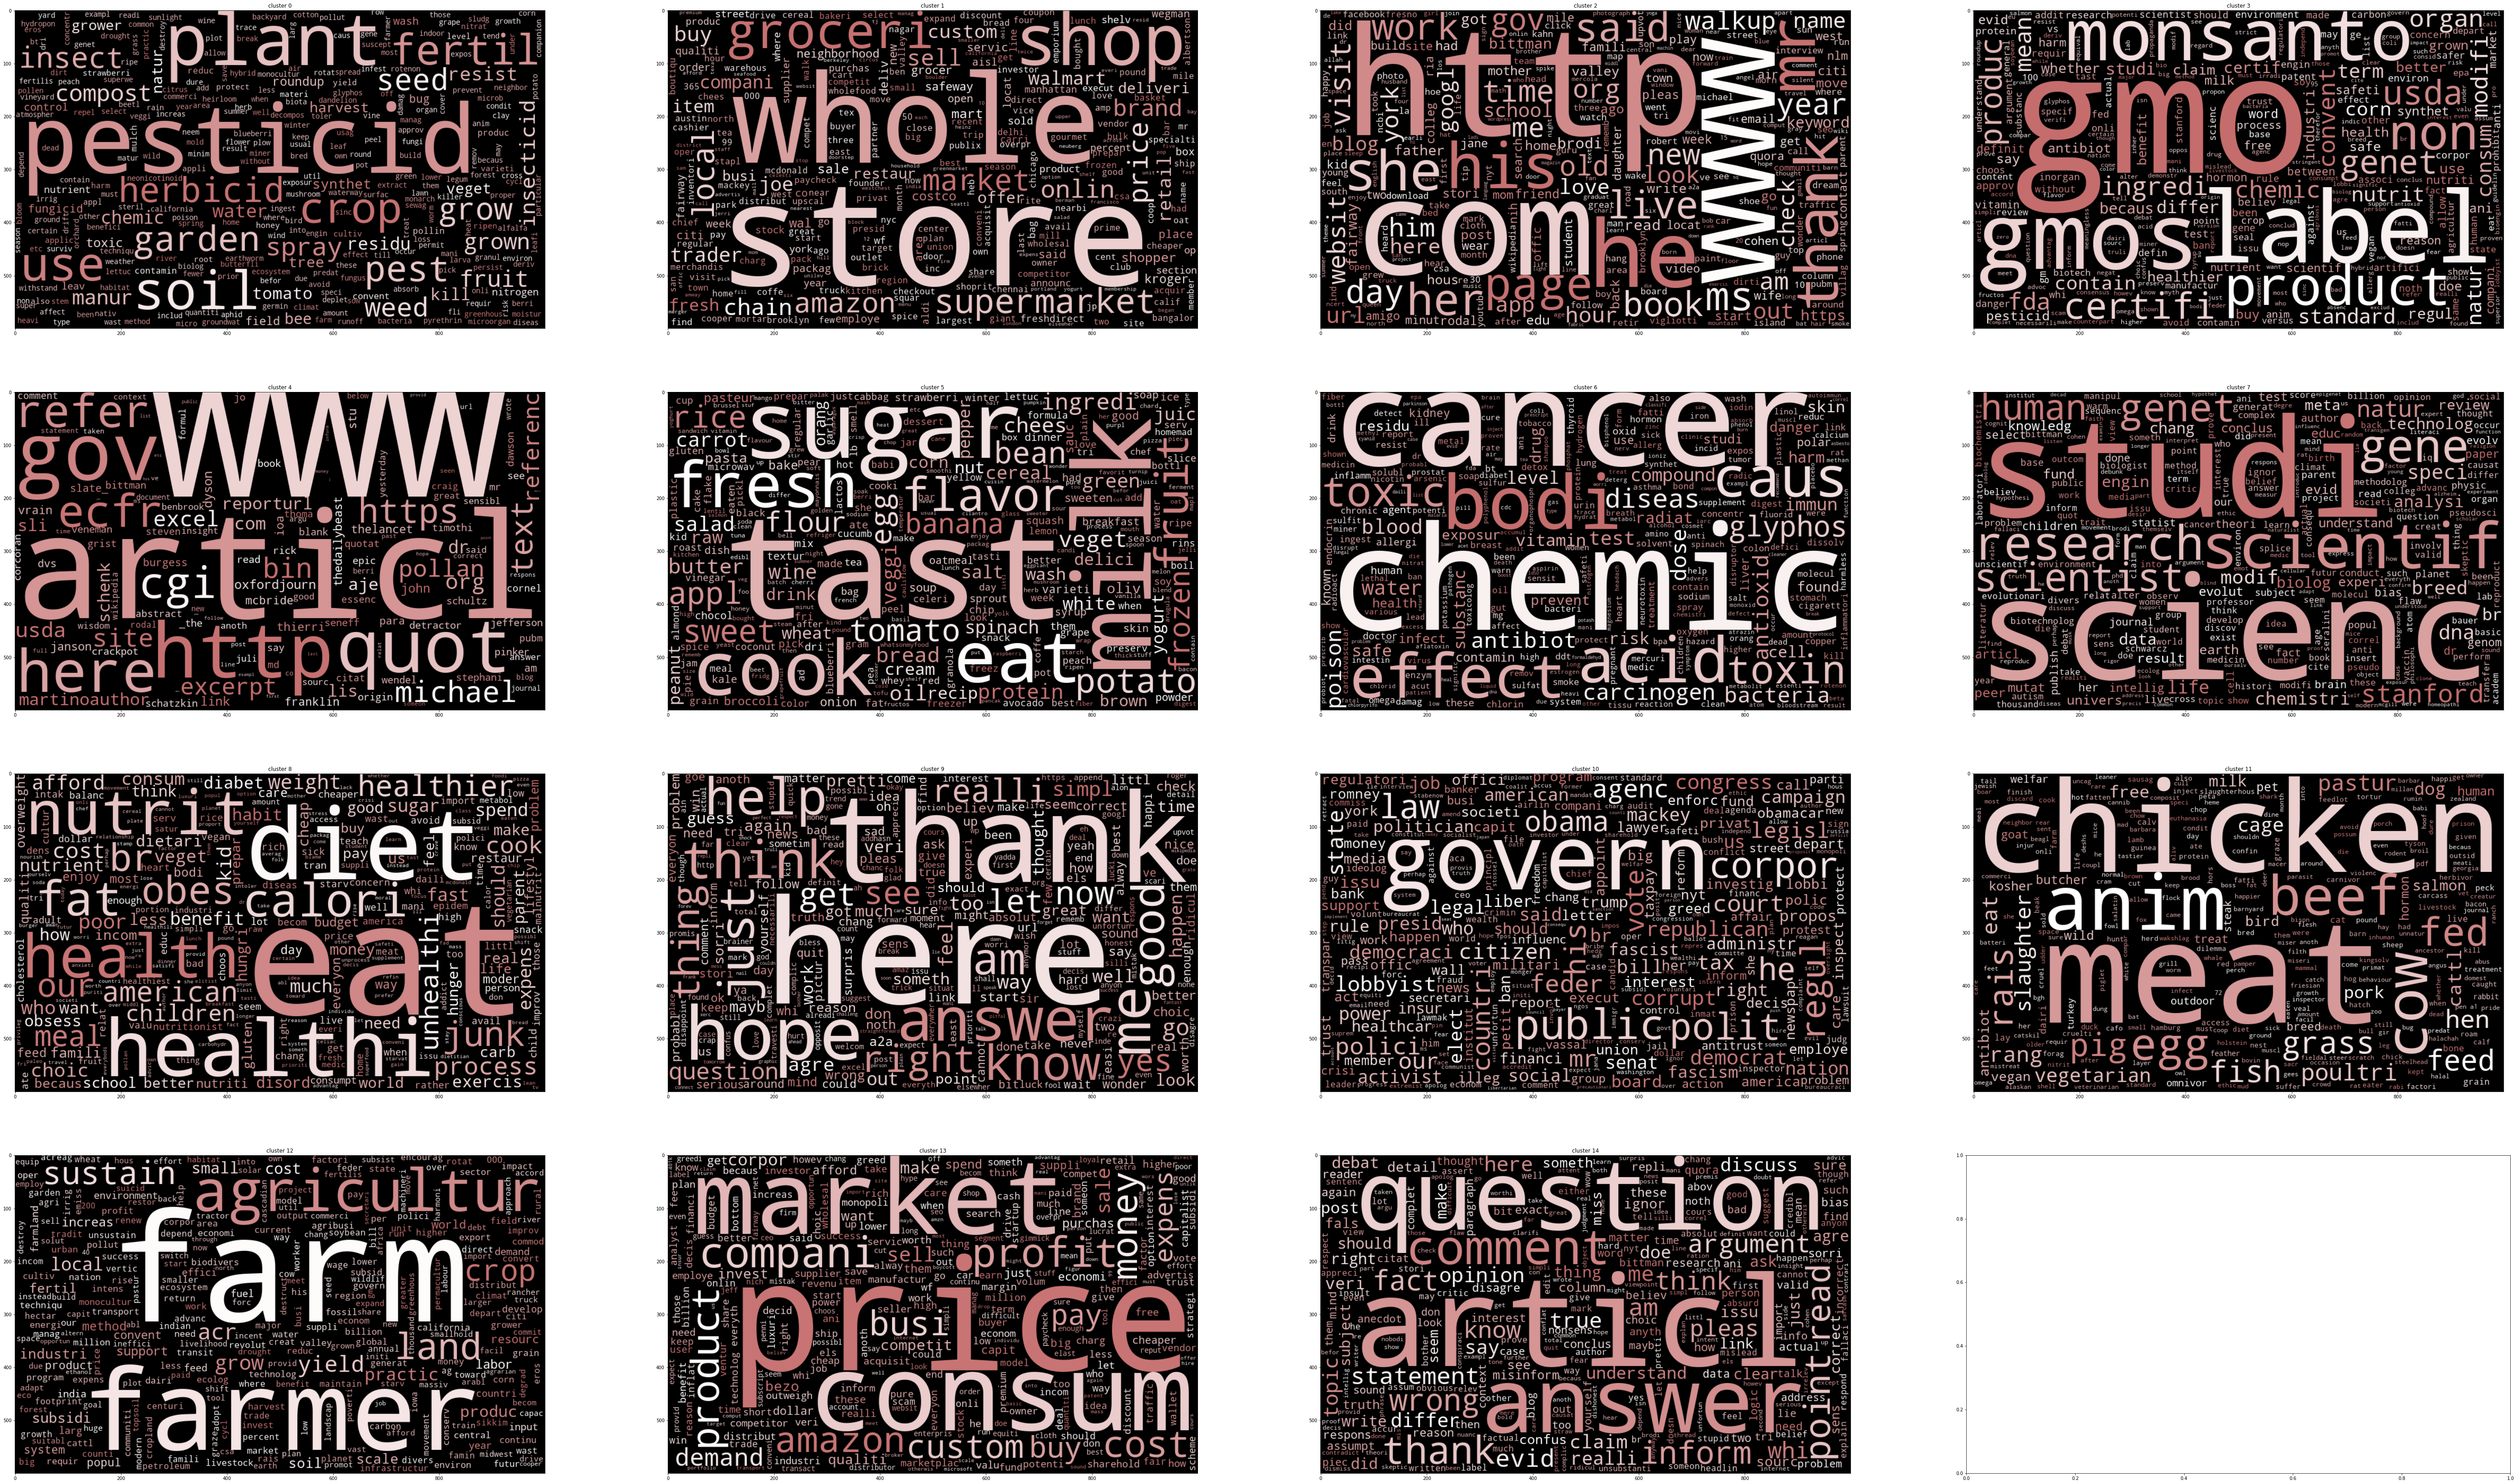
\includegraphics[width=0.45\textwidth]{images/en_15.png}
      \vspace{1em}
      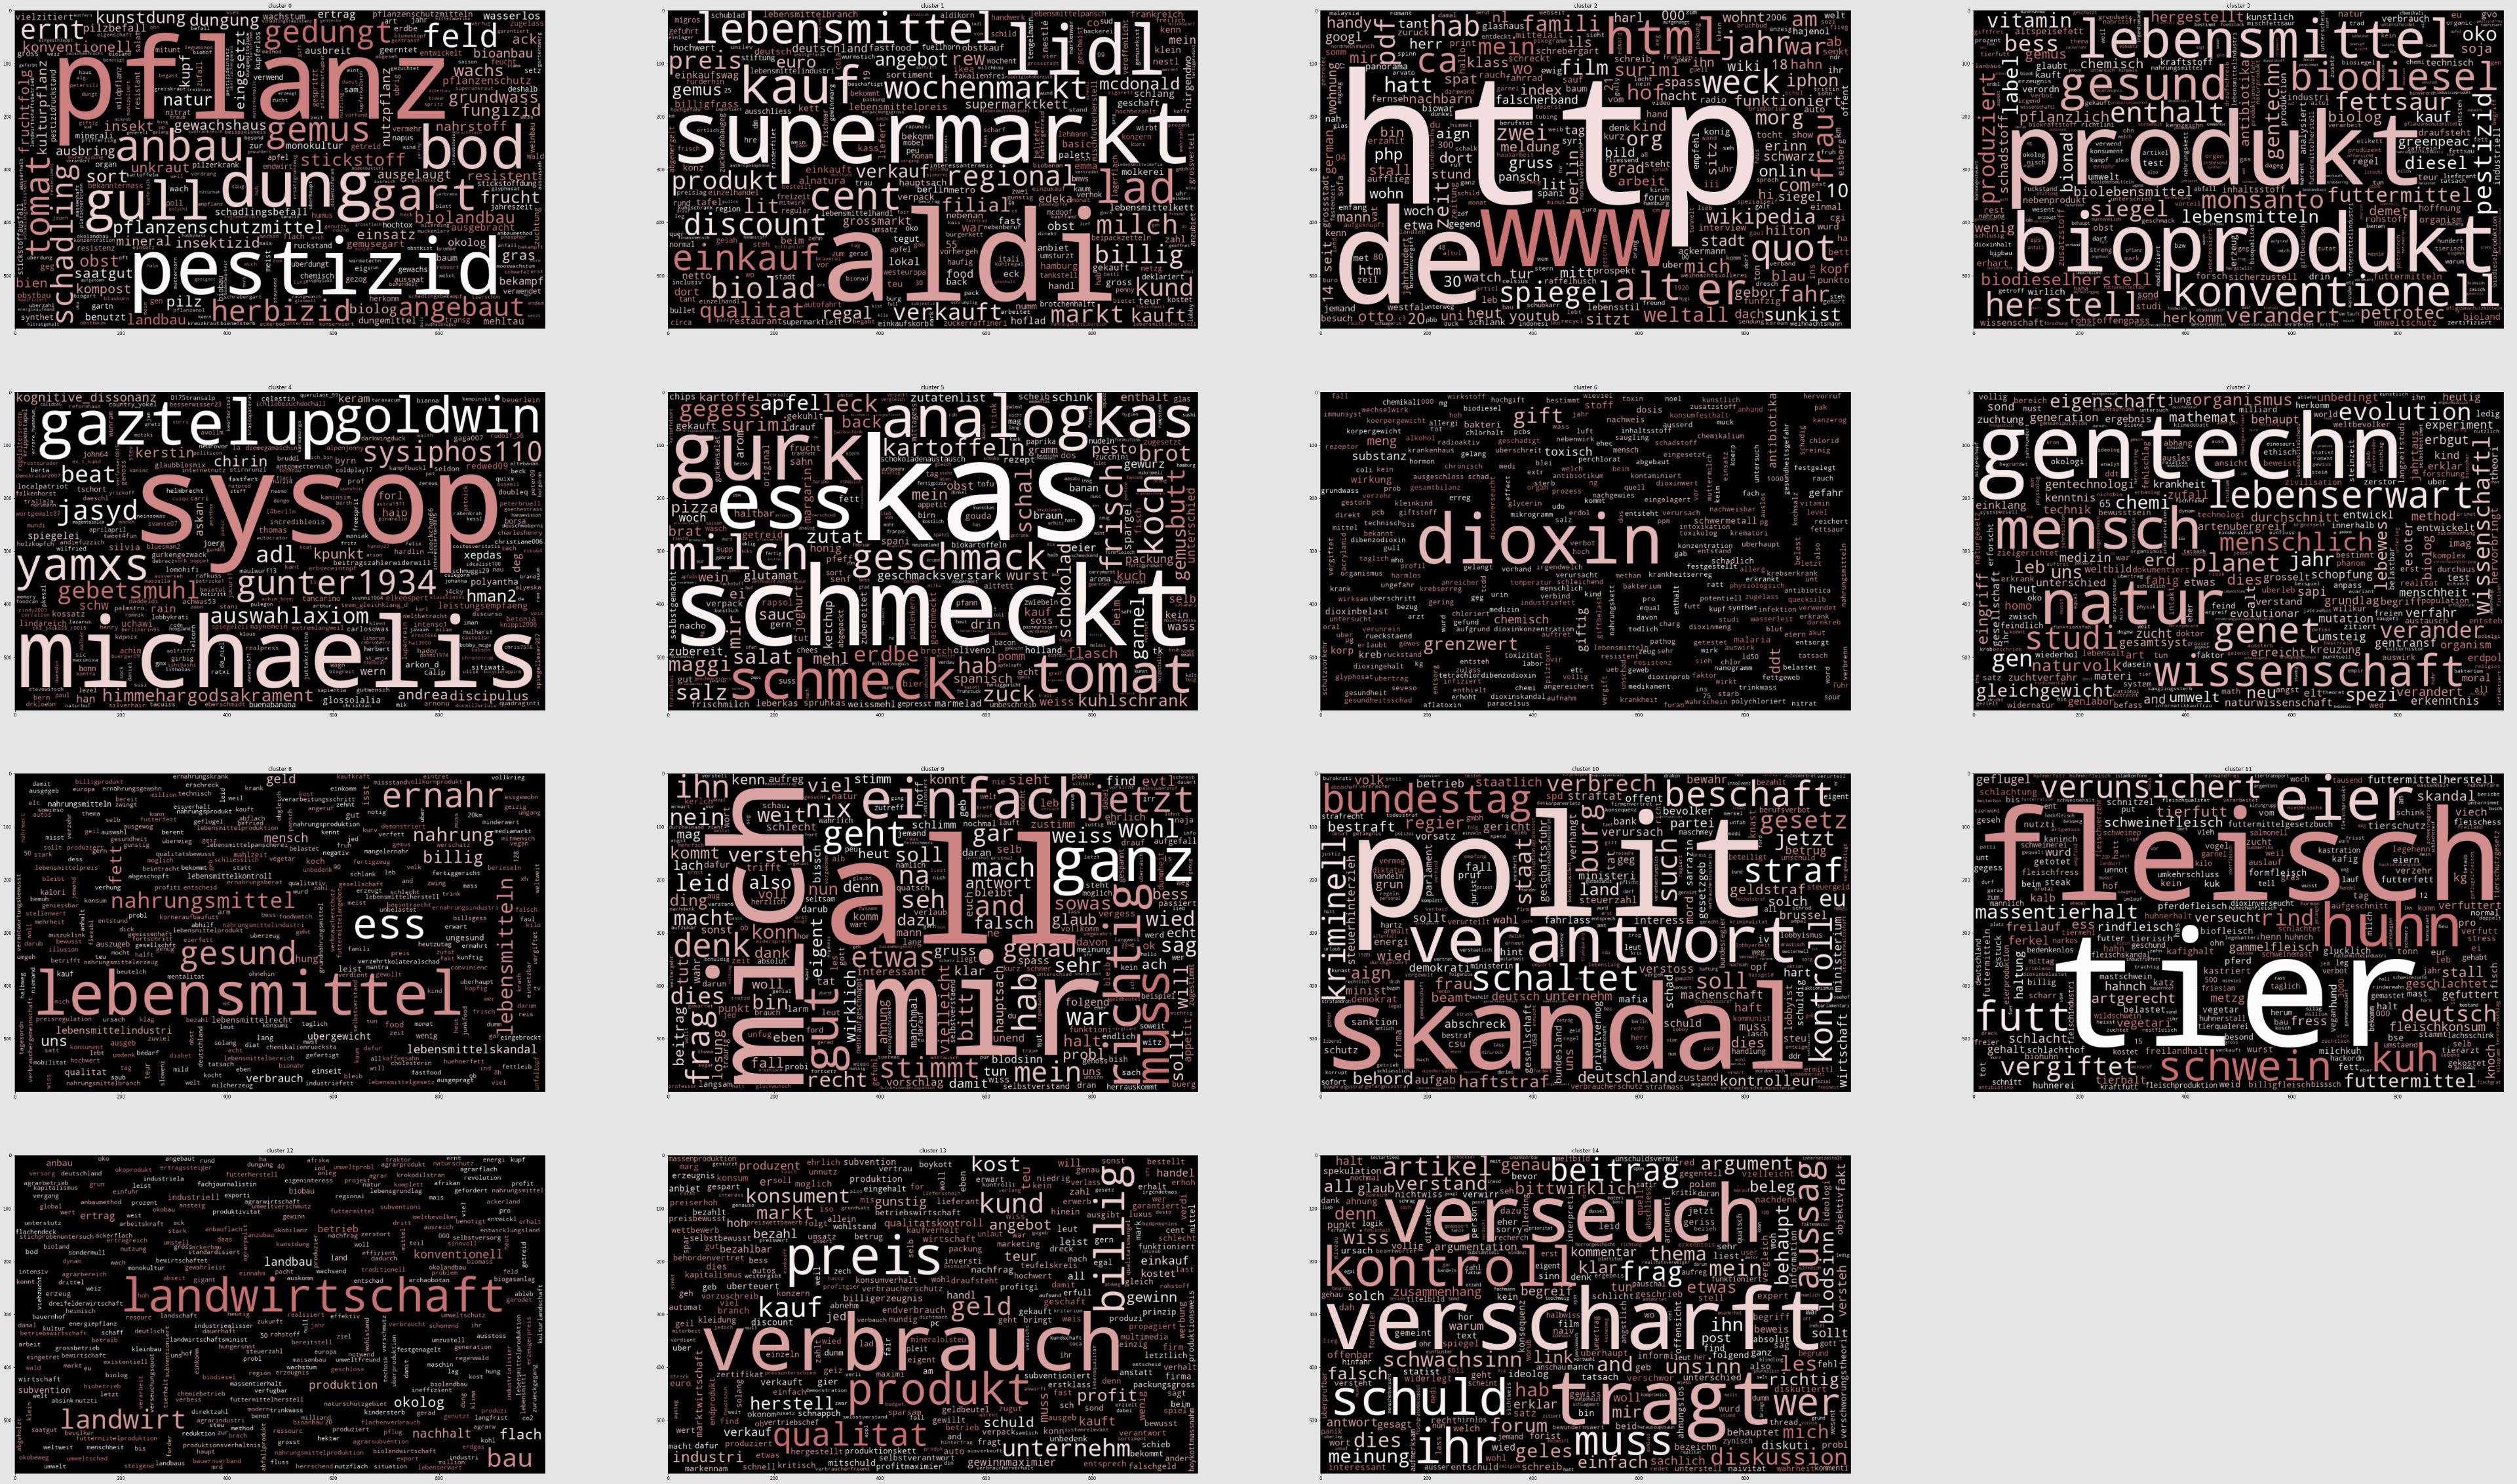
\includegraphics[width=0.45\textwidth]{images/de_15_tfhigh_dim.png}
      \caption{English topwords (left) from NYTimes and Quora & German top words (right) from Die Spiegel}
  \end{figure}
\end{frame}
\end{document}
